\section{Results}
\label{sec:results}

In this evaluation we will be answering the following questions:

\begin{enumerate}
\setlength{\itemsep}{-3pt}  

\item Are there applications/usage scenarios that are supported
efficiently with duty cycling.  What are the power saving achieved by
this approach?

\item What are the power savings achievable with the batching wake up approach?

\item Under what conditions does the wakeup condition approach improve
performance (over the other approaches), and by how much?

\item What are the benefits of having different wake up conditions
(filters)?  Do different applications require different wake up conditions or is
a static wake-up condition sufficient for all applications? 

\item Are the best filter/threshold combinations dependent on the usage
scenario?

\item How sensitive are the energy savings to the configuration thresholds
used in the filter?

\end{enumerate}

\subsection{Energy Savings}

\iffalse
\begin{table*}[t]
    \begin{tabular}{|l|l|l|l|l|l|l|l|}
    \hline
    Action                & Steps & ~    & ~    & ~   & ~   & ~   & ~    \\ \hline
    Recall                & 98\%  & 95\% & 90\% & 55\% & 33\% & 20\% & 11\% \\ \hline
    Always On             & 323   & ~    & ~    & ~   & ~   & ~   & ~    \\ \hline
    Duty Cycling (2 sec)  & ~     & ~    & ~    & 344 & ~   & ~   & ~    \\ \hline
    Duty Cycling (5 sec)  & ~     & ~    & ~    & ~   & 212 & ~   & ~    \\ \hline
    Duty Cycling (10 sec) & ~     & ~    & ~    & ~   & ~   & 131 & ~    \\ \hline
    Duty Cycling (20 sec) & ~     & ~    & ~    & ~   & ~   & ~   & 77.9 \\ \hline
    Batching (2 sec)      & 677   & ~    & ~    & ~   & ~   & ~   & ~    \\ \hline
    Batching (5 sec)      & 328   & ~    & ~    & ~   & ~   & ~   & ~    \\ \hline
    Batching (10 sec)     & 220   & ~    & ~    & ~   & ~   & ~   & ~    \\ \hline
    Batching (20 sec)     & 181   & ~    & ~    & ~   & ~   & ~   & ~    \\ \hline
    Wake-up Condition     & 48.5  & 47.0 & 44.0 & 38.8 & 36.1 & 24.5 & 24.0 \\ \hline
    \end{tabular}
	\caption{Steps - Group 1}
	\label{table:powerProfileNexus}
\end{table*}

\begin{table*}[t]
    \begin{tabular}{|l|l|l|l|l|l|l|l|}
    \hline
    Action                & Steps & ~   & ~   & ~   & ~   & ~   & ~    \\ \hline
    Recall                & 97\%  & 95\% & 90\% & 55\% & 32\% & 20\% & 11\% \\ \hline
    Always On             & 323   & ~   & ~   & ~   & ~   & ~   & ~    \\ \hline
    Duty Cycling (2 sec)  & ~     & ~   & ~   & 344 & ~   & ~   & ~    \\ \hline
    Duty Cycling (5 sec)  & ~     & ~   & ~   & ~   & 212 & ~   & ~    \\ \hline
    Duty Cycling (10 sec) & ~     & ~   & ~   & ~   & ~   & 131 & ~    \\ \hline
    Duty Cycling (20 sec) & ~     & ~   & ~   & ~   & ~   & ~   & 77.9 \\ \hline
    Batching (2 sec)      & 677   & ~   & ~   & ~   & ~   & ~   & ~    \\ \hline
    Batching (5 sec)      & 328   & ~   & ~   & ~   & ~   & ~   & ~    \\ \hline
    Batching (10 sec)     & 220   & ~   & ~   & ~   & ~   & ~   & ~    \\ \hline
    Batching (20 sec)     & 181   & ~   & ~   & ~   & ~   & ~   & ~    \\ \hline
    Wake-up Condition     & 322   & 279 & 227 & 194 & 128 & 112 & 80.5 \\ \hline
    \end{tabular}
	\caption{Steps - Group 3}
	\label{table:powerProfileNexus}
\end{table*}


\begin{table*}[t]
    \begin{tabular}{|l|l|l|l|l|l|l|}
    \hline
    Action                & Transitions & ~    & ~    & ~    & ~    & ~    \\ \hline
    Recall                & 100\%       & 95\% & 90\% & 56\% & 29\% & 15\% \\ \hline
    Always On             & 323         & ~    & ~    & ~    & ~    & ~    \\ \hline
    Duty Cycling (2 sec)  & ~           & ~    & 344  & ~    & ~    & ~    \\ \hline
    Duty Cycling (5 sec)  & ~           & ~    & ~    & 212  & ~    & ~    \\ \hline
    Duty Cycling (10 sec) & ~           & ~    & ~    & ~    & 131  & ~    \\ \hline
    Duty Cycling (20 sec) & ~           & ~    & ~    & ~    & ~    & 77.9 \\ \hline
    Batching (2 sec)      & 677         & ~    & ~    & ~    & ~    & ~    \\ \hline
    Batching (5 sec)      & 328         & ~    & ~    & ~    & ~    & ~    \\ \hline
    Batching (10 sec)     & 220         & ~    & ~    & ~    & ~    & ~    \\ \hline
    Batching (20 sec)     & 181         & ~    & ~    & ~    & ~    & ~    \\ \hline
    Wake-up Condition     & 18.7        & 18.4 & 18.2 & 15.8 & 14.7 & 14.1 \\ \hline
    \end{tabular}
	\caption{Transitions - Group 1}
	\label{table:powerProfileNexus}
\end{table*}

\begin{table*}[t]
    \begin{tabular}{|l|l|l|l|l|l|l|}
    \hline
    Action                & Transitions & ~    & ~    & ~    & ~    & ~    \\ \hline
    Recall                & 100\%       & 95\% & 93\% & 55\% & 33\% & 19\% \\ \hline
    Always On             & 323         & ~    & ~    & ~    & ~    & ~    \\ \hline
    Duty Cycling (2 sec)  & ~           & ~    & 344  & ~    & ~    & ~    \\ \hline
    Duty Cycling (5 sec)  & ~           & ~    & ~    & 212  & ~    & ~    \\ \hline
    Duty Cycling (10 sec) & ~           & ~    & ~    & ~    & 131  & ~    \\ \hline
    Duty Cycling (20 sec) & ~           & ~    & ~    & ~    & ~    & 77.9 \\ \hline
    Batching (2 sec)      & 677         & ~    & ~    & ~    & ~    & ~    \\ \hline
    Batching (5 sec)      & 328         & ~    & ~    & ~    & ~    & ~    \\ \hline
    Batching (10 sec)     & 220         & ~    & ~    & ~    & ~    & ~    \\ \hline
    Batching (20 sec)     & 181         & ~    & ~    & ~    & ~    & ~    \\ \hline
    Wake-up Condition     & 52.4        & 49.8 & 48.6 & 35.5 & 26.3 & 20.4 \\ \hline
    \end{tabular}
	\caption{Transitions - Group 3}
	\label{table:powerProfileNexus}
\end{table*}

\begin{table*}[t]
    \begin{tabular}{|l|l|l|l|l|l|}
    \hline
    Action                & Headbutts & ~   & ~    & ~   & ~   \\ \hline
    Recall                & 100\%     & 57\% & 36\% & 29\% & 14\% \\ \hline
    Always On             & 323       & ~   & ~    & ~   & ~   \\ \hline
    Duty Cycling (2 sec)  & ~         & ~   & ~    & 344 & ~   \\ \hline
    Duty Cycling (5 sec)  & ~         & 212 & ~    & ~   & ~   \\ \hline
    Duty Cycling (10 sec) & ~         & ~   & ~    & ~   & 131 \\ \hline
    Duty Cycling (20 sec) & ~         & ~   & 77.9 & ~   & ~   \\ \hline
    Batching (2 sec)      & 677       & ~   & ~    & ~   & ~   \\ \hline
    Batching (5 sec)      & 328       & ~   & ~    & ~   & ~   \\ \hline
    Batching (10 sec)     & 220       & ~   & ~    & ~   & ~   \\ \hline
    Batching (20 sec)     & 181       & ~   & ~    & ~   & ~   \\ \hline
    Wake-up Condition     & 48.2      & ~   & ~    & ~   & ~   \\ \hline
    \end{tabular}
	\caption{Headbutts - Group 1}
	\label{table:powerProfileNexus}
\end{table*}

\begin{table*}[t]
    \begin{tabular}{|l|l|l|l|l|l|l|}
    \hline
    Action                & Headbutts & ~    & ~    & ~    & ~    & ~    \\ \hline
    Recall                & 100\%     & 95\% & 90\% & 66\% & 40\% & 12\% \\ \hline
    Always On             & 323       & ~    & ~    & ~    & ~    & ~    \\ \hline
    Duty Cycling (2 sec)  & ~         & ~    & ~    & 344  & ~    & ~    \\ \hline
    Duty Cycling (5 sec)  & ~         & ~    & ~    & ~    & 212  & ~    \\ \hline
    Duty Cycling (10 sec) & ~         & ~    & ~    & ~    & 131  & ~    \\ \hline
    Duty Cycling (20 sec) & ~         & ~    & ~    & ~    & ~    & 77.9 \\ \hline
    Batching (2 sec)      & 677       & ~    & ~    & ~    & ~    & ~    \\ \hline
    Batching (5 sec)      & 328       & ~    & ~    & ~    & ~    & ~    \\ \hline
    Batching (10 sec)     & 220       & ~    & ~    & ~    & ~    & ~    \\ \hline
    Batching (20 sec)     & 181       & ~    & ~    & ~    & ~    & ~    \\ \hline
    Wake-up Condition     & 65.8      & 65.6 & 65.6 & 64.9 & 63.2 & 61.2 \\ \hline
    \end{tabular}
	\caption{Headbutts - Group 3}
	\label{table:powerProfileNexus}
\end{table*}
\fi

\begin{table*}[t]
    \begin{tabular}{|l|l|l|l|l|l|l|}
    \hline
	\multirow{2}{*}{~}			& \multirow{2}{*}{Approach}		& \multirow{2}{*}{\parbox{2.2cm}{Sleep Interval (seconds)}}	
																			& \multirow{2}{*}{\parbox{1.2cm}{Power (mW)}} 
																						& \multicolumn{3}{c|}{Recall} 													\\ \cline{5-7}
								&								&			&			& Walking				& Headbutt					& Transitions 				\\ \hline
	\multirow{11}{*}{Group 1}	& \multicolumn{2}{l|}{Always Awake}			& 323		& \multirow{6}{*}{98\%}	& \multirow{6}{*}{100\%}	& \multirow{6}{*}{100\%}	\\ \cline{2-4}
								& \multirow{5}{*}{Batching}		& 2			& 84.0		&						&							&							\\ \cline{3-4}
								& 								& 5			& 60.5		&						&							&							\\ \cline{3-4}
								& 								& 10		& 52.6		&						&							&							\\ \cline{3-4}
								& 								& 20		& 48.7		&						&							&							\\ \cline{3-4}
								& 								& 30		& 47.5		&						&							&							\\ \cline{2-7}
								& \multirow{5}{*}{Duty Cycling}	& 2			& 212		& 94\%					& 57\%						& 100\%						\\ \cline{3-7}
								& 								& 5			& 140		& 82\%					& 14\%						& 35\%						\\ \cline{3-7}
								& 								& 10		& 92.1		& 63\%					& 29\%						& 23\%						\\ \cline{3-7}
								& 								& 20		& 59.4		& 48\%					& 14\%						& 10\%						\\ \cline{3-7}
								& 								& 30		& 44.2		& 31\%					& 7\%						& 4\%						\\ \hline
	\multirow{11}{*}{Group 3}	& \multicolumn{2}{l|}{Always Awake}			& 323		& \multirow{6}{*}{97\%}	& \multirow{6}{*}{100\%}	& \multirow{6}{*}{100\%}	\\ \cline{2-4}
								& \multirow{5}{*}{Batching}		& 2			& 84.0		&						&							&							\\ \cline{3-4}
								& 								& 5			& 60.5		&						&							&							\\ \cline{3-4}
								& 								& 10		& 52.6		&						&							&							\\ \cline{3-4}
								& 								& 20		& 48.7		&						&							&							\\ \cline{3-4}
								& 								& 30		& 47.5		&						&							&							\\ \cline{2-7}
								& \multirow{5}{*}{Duty Cycling}	& 2			& 261		& 89\%					& 47\%						& 90\%						\\ \cline{3-7}
								& 								& 5			& 209		& 76\%					& 28\%						& 39\%						\\ \cline{3-7}
								& 								& 10		& 166		& 64\%					& 27\%						& 8\%						\\ \cline{3-7}
								& 								& 20		& 112		& 42\%					& 19\%						& 7\%						\\ \cline{3-7}
								& 								& 30		& 82.7		& 30\%					& 9\%						& 5\%						\\ \hline
    \end{tabular}
	\caption{Summary of achieved recall and power consumption for the Always On, Duty Cycling and Batching approaches}
	\label{table:summaryAA-DC-BATCHING}
\end{table*}

\begin{table}[t]
    \begin{tabular}{|l|l|l|l|}
	\hline
    ~       					& Action      & Power (mW) & Recall \\ \hline
    \multirow{3}{*}{Group 1} 	& Walking     & 42.2       & 98\%   \\ \cline{2-4}
								& Headbutts   & 42.2       & 100\%  \\ \cline{2-4}
								& Transitions & 15.6       & 100\%  \\ \hline
    \multirow{3}{*}{Group 3} 	& Walking     & 267        & 97\%   \\ \cline{2-4}
								& Headbutts   & 62.7       & 100\%  \\ \cline{2-4}
								& Transitions & 31.1       & 100\%  \\ \hline
    \end{tabular}
	\caption{Summary of achieved recall and power consumption for the Wake-up Conditions approach}
	\label{table:summaryWUC}
\end{table}

\begin{table}[t]
    \begin{tabular}{|l|l|l|l|}
	\hline
    ~       					& Action      & Power (mW) & Recall \\ \hline
    \multirow{3}{*}{Group 1} 	& Walking     & 37.7       & 98\%   \\ \cline{2-4}
								& Headbutts   & 14.1       & 100\%  \\ \cline{2-4}
								& Transitions & 14.9       & 100\%  \\ \hline
	\multirow{3}{*}{Group 2} 	& Walking     & 134        & 99\%   \\ \cline{2-4}
								& Headbutts   & 19.2       & 100\%  \\ \cline{2-4}
								& Transitions & 21.8       & 100\%  \\ \hline
    \multirow{3}{*}{Group 3} 	& Walking     & 240        & 97\%   \\ \cline{2-4}
								& Headbutts   & 19.7       & 100\%  \\ \cline{2-4}
								& Transitions & 24.6       & 100\%  \\ \hline
    \end{tabular}
	\caption{Recall and power consumption for a perfect Wake-up Condition (Oracle)}
	\label{table:WUCoracle}
\end{table}

This section answers the first three questions. Table \ref{table:summaryAA-DC-BATCHING} summarizes the power and event of interest recall data for the always on scenario and for various wake-up intervals for the duty cycling and batching approaches. Similarly, Table \ref{table:summaryWUC} summarizes the results for the approach that uses wake-up conditions. The information in this figure represents the best wake-up conditions in terms of power consumption that achieved the same recall as the always on scenario.

We note the following:

The duty cycling approach has significant power savings for sleep intervals greater than 5 seconds, compared to the always on scenario. However, in cases where the event of interests occurs rarely (group 1), the power savings of duty cycling are suboptimal because of numerous wake-up that result in no events of interest being detected. The greatest drawback of this approach is that it is not appropriate for applications that requires a high event of interest recall. Using a 5-second sleep interval, the highest achieved recall was 56%, for the transitions action in group 1.

The batching approach achieves the same event of interest recalls as the always on scenario, and is able to reduce power consumption for sleep intervals greater than 5 seconds. Shorter wake-up intervals can potentially cause more energy consumption than the Always Awake case because of the additional energy cost of transitioning between the sleep and awake states. Note that increasing the wake-up interval has diminishing power saving returns. A lower bound to the power consumption of the entire system is the sum of the power consumed by the main device while sleeping and the peripheral processor while being awake. Compared to the other approaches, batching has the best power savings for use cases where the event of interest occurs very frequently (i.e. walking in group 3). However, if the event of interest occurs very infrequently, batching suffers from the same problem as duty cycling. Its power consumption becomes suboptimal because of a large number of wake-ups that do not result in an event of interest being detected. In this approach, events of interest are only detected after the main processor wakes up. As a result, the delay between the time when the event is occurring and the time when it is detected can be as long as the batching interval. Therefore, this approach may not be appropriate for applications that are expected to react immediately after an event of interest occurs. For example, the user of a gesture recognition application would not be satisfied if the application detects the performed gesture after a delay of more than a couple of seconds.

The wake-up conditions approach has the lowest power consumption in every scenario other than step detection in group 3. All these scenarios are similar in that the event of interest occurs infrequently (less than 15% of the time, as seen in Figure \ref{fig:fig:actionTimes}). The lower bound for power consumption is the sum of the power consumed by the main device while sleeping and the peripheral processor while being awake. For our prototype this value is 13.3 mW (9.7 mW for the Nexus 4 and 3.6 mW for the TI MSP430 microcontroller. When attempting to detect transition in group 1, the system is estimated to consume 18.7 mW which achieving 100% recall. This equates to 97.1% of the total potential power savings compared to the always on approach.

\subsection{Predefined action vs predefined filter}

\begin{table*}[t]
    \begin{tabular}{|l|l|l|l|l|l|l|l|}
    \hline
    \multirow{2}{*}{ Wake-up condition used}
							& \multirow{2}{*}{~}	& \multicolumn{3}{c|}{Headbutts} 	& \multicolumn{3}{c|}{Transitions} 	\\ \cline{2-8}
							&						& Group 1 	& Group 2	& Group 3 	& Group 1 	& Group 2	& Group 3 	\\ \hline
    \multirow{2}{*}{Best for step detection}
							& Recall 				& 35.7\%  	& 62.7\%    & 69.3\%  	& 87.5\% 	& 76.4\%	& 78.3\%  	\\ \cline{2-8}
							& Power  				& 42.2 		& 154       & 267     	& 42.2 		& 154		& 267     	\\ \hline
    \multirow{2}{*}{Best custom}
							& Recall 				& 100\%   	& 100\%     & 100\%   	& 100\%   	& 100\%		& 100\%   	\\ \cline{2-8}
							& Power  				& 42.2   	& 62.4      & 62.7    	& 15.7    	& 27.2		& 31.1    	\\ \hline
    \end{tabular}
	\caption{Detection recall and power consumption for the Headbutts and Transitions actions using fixed or custom wake-up conditions}
	\label{table:predifinedActionVsPredefinedFilter}
\end{table*}

This section answers question 4. For this purpose, we assume that step detection is the one action that our hardware supports and we compare that with the benefits of custom filters for each of the other 2 applications. 

We start off by selecting the best wake-up condition for step detection. We used this wake-up condition and attempted to detect headbutts and stance transitions. The top part Table \ref{table:predifinedActionVsPredefinedFilter} shows the results in terms or detection recall and power consumption. The bottom half of the table shows the results for the same metrics when we used the best wake-up condition for those specific actions. We note that in every single case, using a custom filter increased detection recall. For the headbutt action, recall was more than doubled for every group. For transitions, using a custom filter increased recall to 100% for every group. In terms of power consumption the best results are visible in group 3, the group with the highest amount of walking. In group 3, the energy consumption was reduced by up to 84%.

We can conclude that using a fixed wake-up condition (or a hardware supported action) may work very well for a small set of application, but is extremely inefficient for most other applications. As such, developers should be able to configure the wake-up conditions based on the needs of their application. 

\subsection{Usage Dependence}

\begin{figure}[h]
	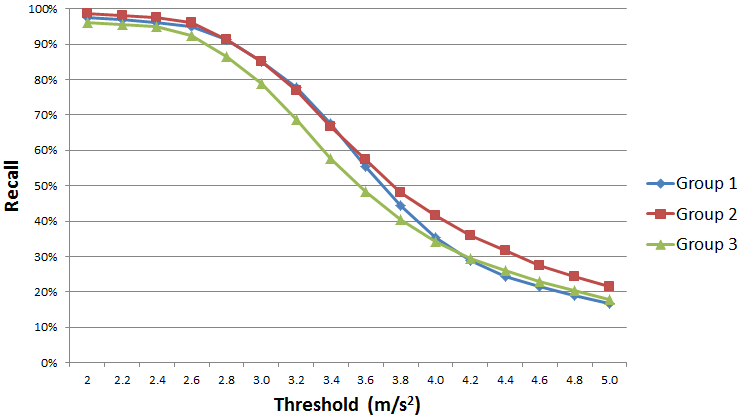
\includegraphics[width=8.5cm]{wuc_steps_recall_by_group_and_th.png}
	\caption{}
    \label{fig:wucStepsRecallByGroupAndThreshold}
\end{figure}

This section answers question 5. Figure \ref{fig:wucStepsRecallByGroupAndThreshold} shows the step recall based on the wake-up condition threshold value for each of the groups. We note that for different usage scenarios (i.e. each of the groups) the recall does not change by more than 10% for any given threshold. Similar results were found for all the events of interest. 

We conclude that the best filter and threshold combinations are not dependent on the usage scenario.


\subsection{Threshold Sensitivity}

\begin{figure}[h]
	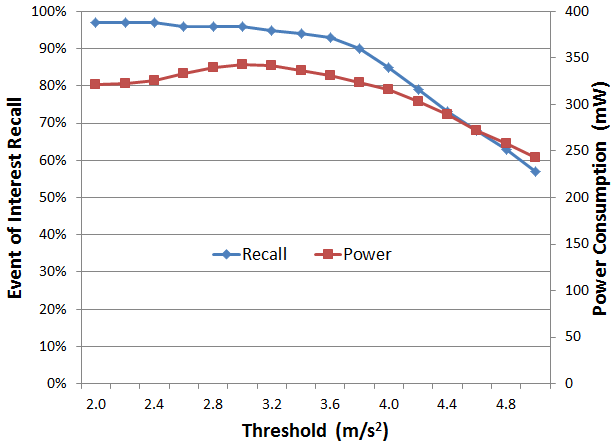
\includegraphics[width=8.5cm]{wuc_step_th_group3.png}
	\caption{}
    \label{fig:wucStepThRecallPowerGroup2}
\end{figure}

\begin{figure}[h]
	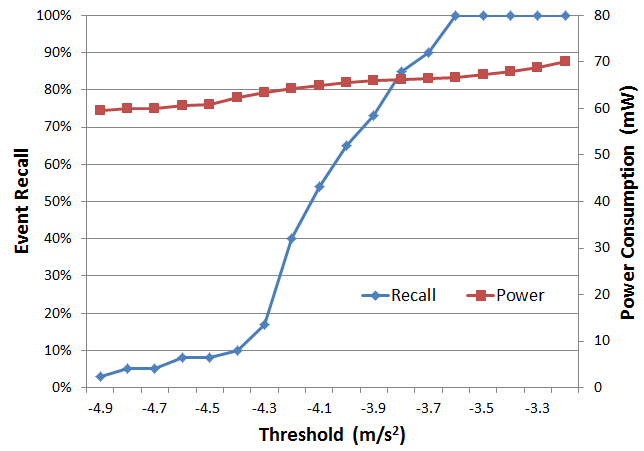
\includegraphics[width=8.5cm]{wuc_hb_fft_group3.png}
	\caption{}
    \label{fig:wucHbFftRecallPowerGroup3}
\end{figure}

\begin{figure}[h]
	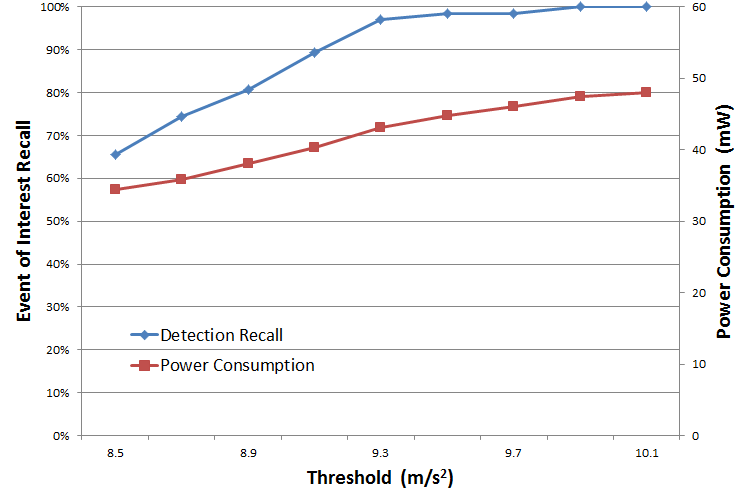
\includegraphics[width=8.5cm]{wuc_trans_ema_group2.png}
	\caption{}
    \label{fig:wucTransEmaRecallPowerGroup2}
\end{figure}


This section answers question 6. Figures \ref{fig:wucStepThRecallPowerGroup2}, \ref{fig:wucHbFftRecallPowerGroup3} and \ref{fig:wucTransEmaRecallPowerGroup3} show the detection recall and power consumption for each application using the best wake-up condition for that specific application. From the figures we note that the choice of threshold is very important, as choosing a threshold that is too strict will cause a significant drop-off in the achieved recall. However, choosing a threshold that is too lenient will result in additional power consumption without any extra benefit to recall because of unnecessary wake-ups. 

TODO: the choice of threshold seems forgiving, but I'm not sure how to explain it